% !TeX program = lualatex
% ============================================================
%  Presentazione di tesi -- EggLog Motion Core
%  Tema: Padova (rosso istituzionale Pantone 1807, #9B0014)
%  Compilare con LUALATEX (necessario per fontspec/Carlito)
% ============================================================
\documentclass[aspectratio=169]{beamer}
\usetheme{Padova}

\usepackage{tcolorbox}
\tcbuselibrary{skins,raster}
\usepackage{pgfplots}
\pgfplotsset{compat=1.18}
\usepackage{booktabs}
\usepackage{pifont}
\usetikzlibrary{arrows.meta,decorations.pathreplacing,shapes.geometric}

\title[EggLog Motion Core]{Evoluzione e ottimizzazione di un firmware embedded\\per un sistema di telemetria basato su ESP32}
\subtitle{EggLog Motion Core -- telemetria per il motorsport motociclistico}
\author{Zakaria Laoud}
\relatore{Nome Cognome}
\date{Anno Accademico 2025/2026}

\padovalogowhite{assets/logo_unipd_bianco.png}
\padovalogored{assets/logo_unipd_rosso.png}

\newtcolorbox{cardred}[1]{colback=padovaredpale,colframe=padovared,boxrule=0.5pt,arc=2pt,
  fonttitle=\bfseries\small,coltitle=white,colbacktitle=padovared,title=#1,
  left=5pt,right=5pt,top=3pt,bottom=3pt}
\newtcolorbox{cardpetrol}[1]{colback=padovapetrollight,colframe=padovapetrol,boxrule=0.5pt,arc=2pt,
  fonttitle=\bfseries\small,coltitle=white,colbacktitle=padovapetrol,title=#1,
  left=5pt,right=5pt,top=3pt,bottom=3pt}

\begin{document}

\maketitle

\begin{frame}{Indice}
  \tableofcontents
\end{frame}

\section{Introduzione}

\begin{frame}{L'azienda e il progetto}
  \begin{columns}[T,onlytextwidth]
    \begin{column}{0.46\textwidth}
      \vspace{2pt}
      \begin{center}
        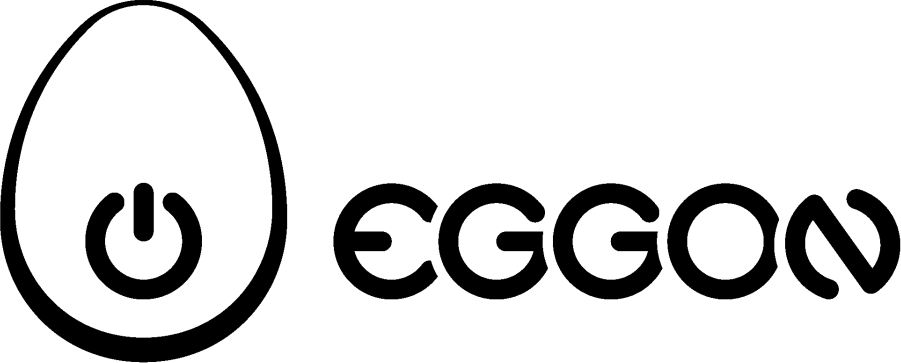
\includegraphics[width=0.92\textwidth]{assets/eggon_logo_black.png}
      \end{center}
      \vspace{6pt}
      \begin{itemize}
        \item \textbf{Software house} padovana attiva in Digital Health, IIoT, Fintech
        \item Team \textbf{giovane}, nato da esperienza maturata negli \textbf{USA}
      \end{itemize}
    \end{column}
    \begin{column}{0.5\textwidth}
      \begin{block}{Il progetto: EggLog Motion Core}
        \begin{itemize}
          \item Telemetria per il \textbf{motorsport motociclistico}
          \item \textbf{Firmware ESP32} + app mobile companion
        \end{itemize}
      \end{block}
    \end{column}
  \end{columns}
\end{frame}

\begin{frame}{Motivazioni della scelta del progetto}
  \begin{center}
  \begin{tcbraster}[raster columns=2,raster rows=2,raster equal height,raster column skip=8pt,raster row skip=8pt]
    \begin{cardred}{IoT ed embedded}
      Passione coltivata fin dalle \textbf{scuole superiori}
    \end{cardred}
    \begin{cardred}{Automotive}
      Interesse per \textbf{telemetria} e reti veicolari
    \end{cardred}
    \begin{cardpetrol}{Ambiente giovane}
      Comunicazione \textbf{diretta}, confronto continuo
    \end{cardpetrol}
    \begin{cardpetrol}{Sfida tecnica}
      Firmware più \textbf{strutturato}, crescita personale
    \end{cardpetrol}
  \end{tcbraster}
  \end{center}
\end{frame}

\section{Contesto e obiettivi}

\begin{frame}{Il contesto: sistema esistente e vincoli}
  \begin{columns}[T,onlytextwidth]
    \begin{column}{0.5\textwidth}
      \begin{block}{Sistema esistente}
        \begin{itemize}
          \item Dati salvati in \textbf{file CSV multipli} su SD
          \item Architettura \textbf{producer-consumer} con \textbf{ping-pong buffer}
        \end{itemize}
      \end{block}
    \end{column}
    \begin{column}{0.5\textwidth}
      \begin{alertblock}{Vincoli di progetto}
        \begin{itemize}
          \item Microcontrollore \textbf{ESP32-S3}, firmware in \textbf{C/C++}
          \item \textbf{Sniffer CAN separato}, bus in modalità \textbf{listen-only}
        \end{itemize}
      \end{alertblock}
    \end{column}
  \end{columns}
\end{frame}

\begin{frame}{Tecnologie utilizzate}
  \begin{center}
    \begin{columns}[T,onlytextwidth]
      \begin{column}{0.48\textwidth}
        \centering
        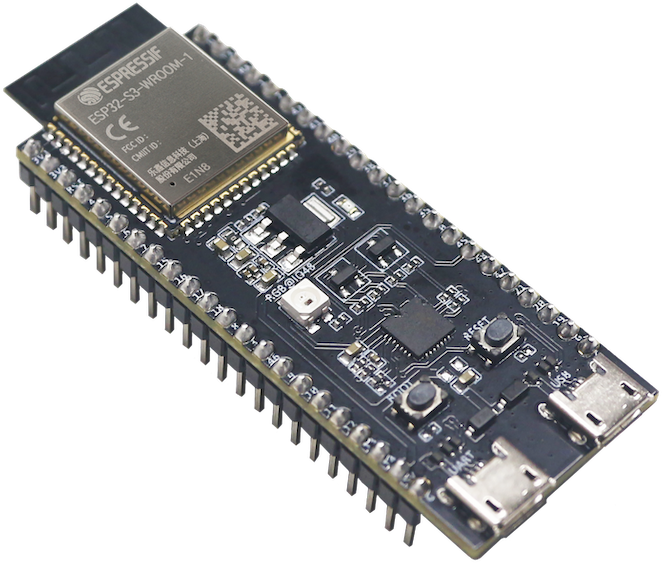
\includegraphics[height=2.7cm]{assets/esp32s3.png}\\[2pt]
        {\scriptsize ESP32-S3-DevKitC-1}
      \end{column}
      \begin{column}{0.48\textwidth}
        \centering
        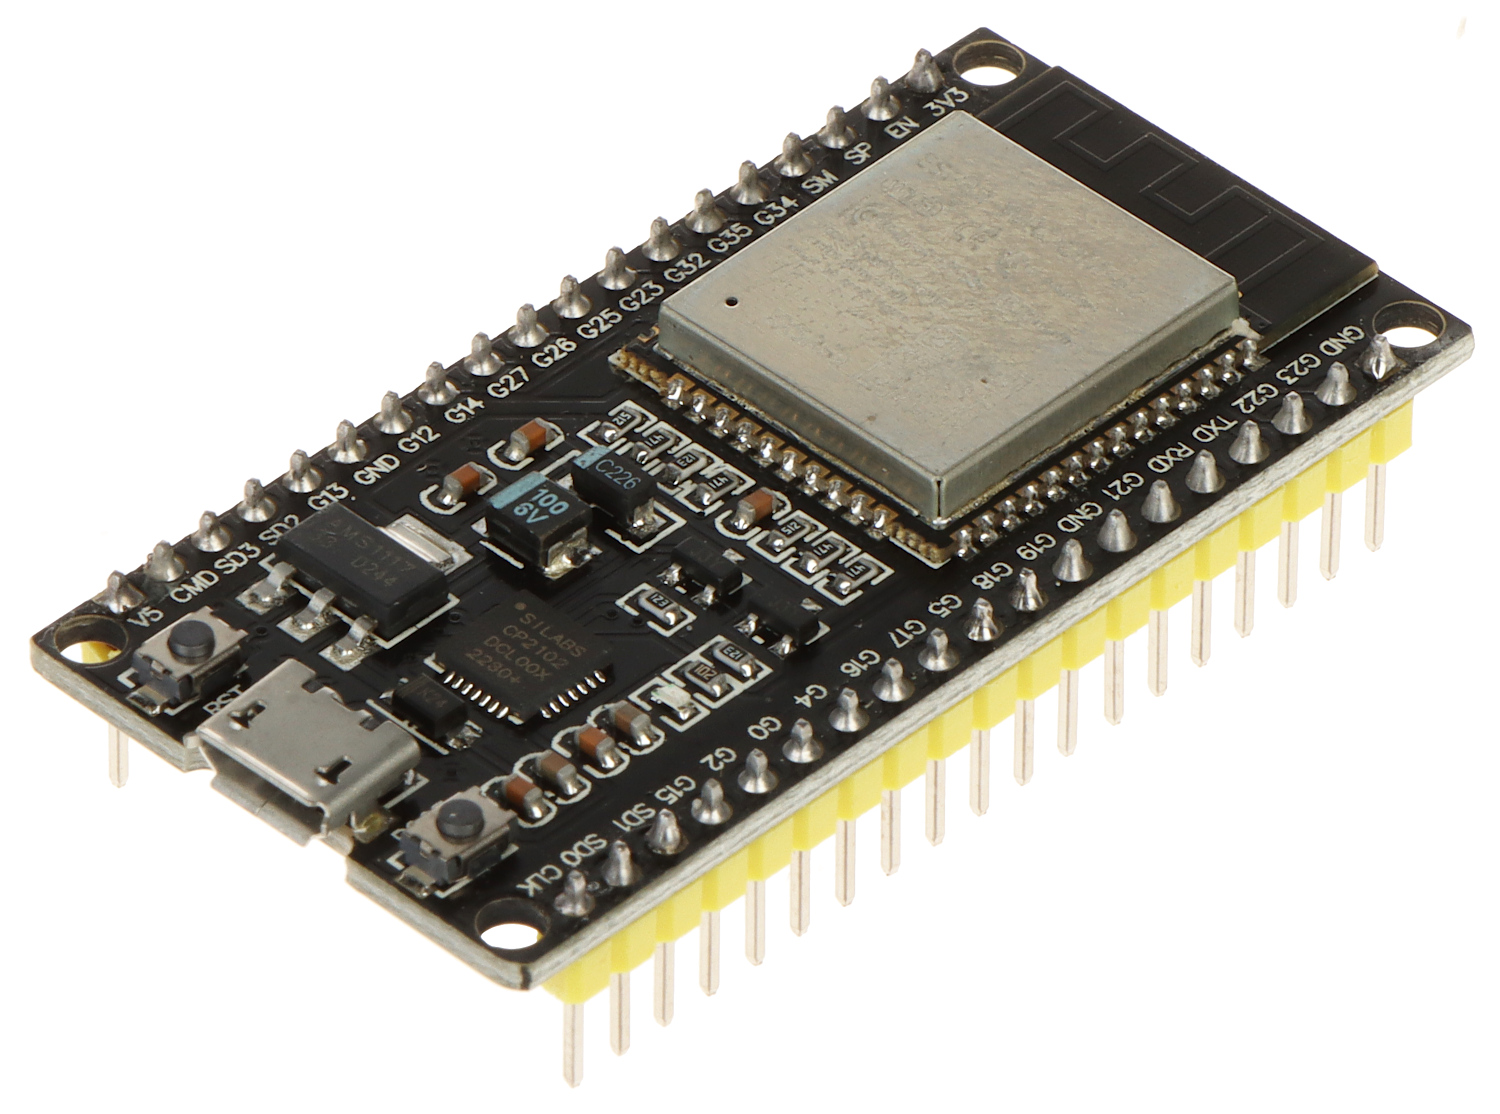
\includegraphics[height=2.7cm]{assets/esp32wroom.jpeg}\\[2pt]
        {\scriptsize ESP-WROOM-32}
      \end{column}
    \end{columns}
  \end{center}
  \vspace{8pt}
  \begin{columns}[T,onlytextwidth]
    \begin{column}{0.5\textwidth}
      \begin{itemize}
        \item \textbf{C++20} su ESP32 Arduino Core con \textbf{FreeRTOS}
        \item App companion in \textbf{React Native / TypeScript}
      \end{itemize}
    \end{column}
    \begin{column}{0.5\textwidth}
      \begin{itemize}
        \item Versionamento con \textbf{Git}, build con \textbf{PlatformIO}
        \item Documentazione con \textbf{PlantUML} e modello \textbf{C4}
      \end{itemize}
    \end{column}
  \end{columns}
\end{frame}

\begin{frame}{Obiettivi dello stage}
  \begin{center}
  \begin{tcbraster}[raster columns=3,raster equal height,raster column skip=8pt]
    \begin{cardred}{\centering Obbligatori}
      \centering{\Huge\bfseries 9}\\[4pt]
      \small refactoring storage, formato binario, recovery
    \end{cardred}
    \begin{cardred}{\centering Desiderabili}
      \centering{\Huge\bfseries 3}\\[4pt]
      \small modello 3D, dati ECU, avviso SD
    \end{cardred}
    \begin{cardred}{\centering Facoltativi}
      \centering{\Huge\bfseries 2}\\[4pt]
      \small indicizzazione sessioni, gestione inattività
    \end{cardred}
  \end{tcbraster}
  \end{center}
\end{frame}

\section{Lavoro svolto}

\begin{frame}{Superfile: il nuovo sistema di persistenza}
  \begin{center}
  \begin{tikzpicture}[font=\small]
    \def\w{10.4} \def\h{1.0}
    \draw[fill=padovareddark,draw=none] (0,0) rectangle (1.3,\h);
    \node[white,font=\bfseries\scriptsize] at (0.65,\h/2) {Header};
    \draw[fill=padovared,draw=none] (1.3,0) rectangle (6.8,\h);
    \node[white,font=\scriptsize] at (4.05,\h/2) {Dati validi (buffer circolare)};
    \draw[fill=padovagold,draw=none] (6.8,0) rectangle (8.5,\h);
    \node[white,font=\tiny,align=center] at (7.65,\h/2) {Finestra\\pre-azzerata};
    \draw[fill=padovagraylight,draw=none] (8.5,0) rectangle (\w,\h);
    \node[padovaink,font=\scriptsize] at (9.45,\h/2) {Libero};
    \draw[draw=padovaink,line width=0.6pt] (0,0) rectangle (\w,\h);
    \foreach \x in {1.3,6.8,8.5} \draw[draw=padovabg,line width=1pt] (\x,0)--(\x,\h);
    \draw[-{Latex[length=2mm]},padovaink,line width=0.8pt]
      (\w+0.55,\h*0.82) arc[start angle=15,end angle=330,radius=0.32];
    \node[padovaink,font=\tiny,align=left,anchor=west] at (\w+0.95,\h*0.5) {scrittura\\circolare};
  \end{tikzpicture}
  \end{center}
  \vspace{2pt}
  \begin{itemize}
    \item Sostituisce \textbf{tanti file CSV} con \textbf{un unico file} per sensore
    \item \textbf{Buffer circolare} preallocato: zero frammentazione
    \item \textbf{Finestra pre-azzerata} $\rightarrow$ recovery automatico dopo crash
    \item Formato \textbf{binario compatto}: più campioni per byte
  \end{itemize}
\end{frame}

\begin{frame}{Stato del dispositivo, LED e gestione sessione}
  \begin{columns}[T,onlytextwidth]
    \begin{column}{0.44\textwidth}
      \begin{tikzpicture}[font=\small]
        \foreach \i/\col/\txt in {0/red/Errore o SD mancante,1/blue/Pairing BLE in corso,2/padovagold/Calibrazione IMU,3/padovapetrol/Sessione sospesa}{
          \node[draw=none,fill=\col,circle,minimum size=9pt] at (0,-0.75*\i) {};
          \node[anchor=west,font=\scriptsize] at (0.35,-0.75*\i) {\txt};
        }
      \end{tikzpicture}
    \end{column}
    \begin{column}{0.53\textwidth}
      \begin{itemize}
        \item Stato del dispositivo \textbf{centralizzato} (STAND\_BY, LOGGING, SUSPENDED\dots)
        \item LED con \textbf{priorità esplicita} tra stati concorrenti
        \item Sensori attivi \textbf{solo durante la sessione}
        \item Comandi \textbf{START/STOP} via BLE per avvio e arresto
      \end{itemize}
    \end{column}
  \end{columns}
\end{frame}

\begin{frame}{Calibrazione dei sensori}
  \begin{center}
  \begin{tikzpicture}[font=\scriptsize,
      box/.style={draw=padovared,fill=padovaredpale,rounded corners=2pt,minimum width=3.1cm,minimum height=1.3cm,align=center,font=\small}]
    \node[box] (s1) at (0,0) {1. Moto\\in verticale};
    \node[box] (s2) at (4.2,0) {2. Moto\\inclinata a destra};
    \node[box] (s3) at (8.4,0) {3. Salvataggio\\calibrazione};
    \draw[-{Latex[length=2.5mm]},padovared,line width=1pt] (s1)--(s2);
    \draw[-{Latex[length=2.5mm]},padovared,line width=1pt] (s2)--(s3);
  \end{tikzpicture}
  \end{center}
  \vspace{6pt}
  \begin{itemize}
    \item \textbf{Barometro} più preciso del GPS in quota (2 m contro 25 m)
    \item Calibrazione altitudine tramite \textbf{mediana} dei campioni
    \item \textbf{IMU}: calibrazione guidata in \textbf{3 passaggi}
    \item Macchina a stati con \textbf{retry isolato} per singolo step
  \end{itemize}
\end{frame}

\begin{frame}{EggLog CAN Sniffer}
  \begin{center}
  \begin{tikzpicture}[font=\scriptsize,
      box/.style={draw=padovapetrol,fill=padovapetrollight,rounded corners=2pt,minimum width=3.0cm,minimum height=1.2cm,align=center,font=\small}]
    \node[box] (ecu) at (0,0) {Bus CAN\\della moto};
    \node[box] (sniffer) at (4.6,0) {EggLog\\CAN Sniffer};
    \node[box] (app) at (9.2,0) {EggLog\\Motion Core};
    \draw[-{Latex[length=2.5mm]},padovapetrol,line width=1pt] (ecu)--(sniffer)
      node[midway,above,font=\tiny]{listen-only + TVS};
    \draw[-{Latex[length=2.5mm]},padovapetrol,line width=1pt] (sniffer)--(app)
      node[midway,above,font=\tiny]{BLE advertising};
  \end{tikzpicture}
  \end{center}
  \vspace{6pt}
  \begin{itemize}
    \item Nodo \textbf{separato}, nessun collegamento elettrico diretto
    \item Bus CAN in modalità \textbf{listen-only}: zero interferenza
    \item Protezione \textbf{TVS} sulle linee CAN\_H / CAN\_L
    \item Dati trasmessi via \textbf{BLE advertising broadcast}
  \end{itemize}
\end{frame}

\begin{frame}{Applicazione mobile: nuove funzionalità}
  \begin{columns}[T,onlytextwidth]
    \begin{column}{0.42\textwidth}
      \begin{itemize}
        \item \textbf{Modello 3D} del veicolo in tempo reale
        \item Rendering \textbf{disaccoppiato} dal ciclo BLE
        \item Avviso di \textbf{microSD mancante}
        \item Configurazione dei \textbf{parametri} via app
      \end{itemize}
    \end{column}
    \begin{column}{0.4\textwidth}
      \centering
      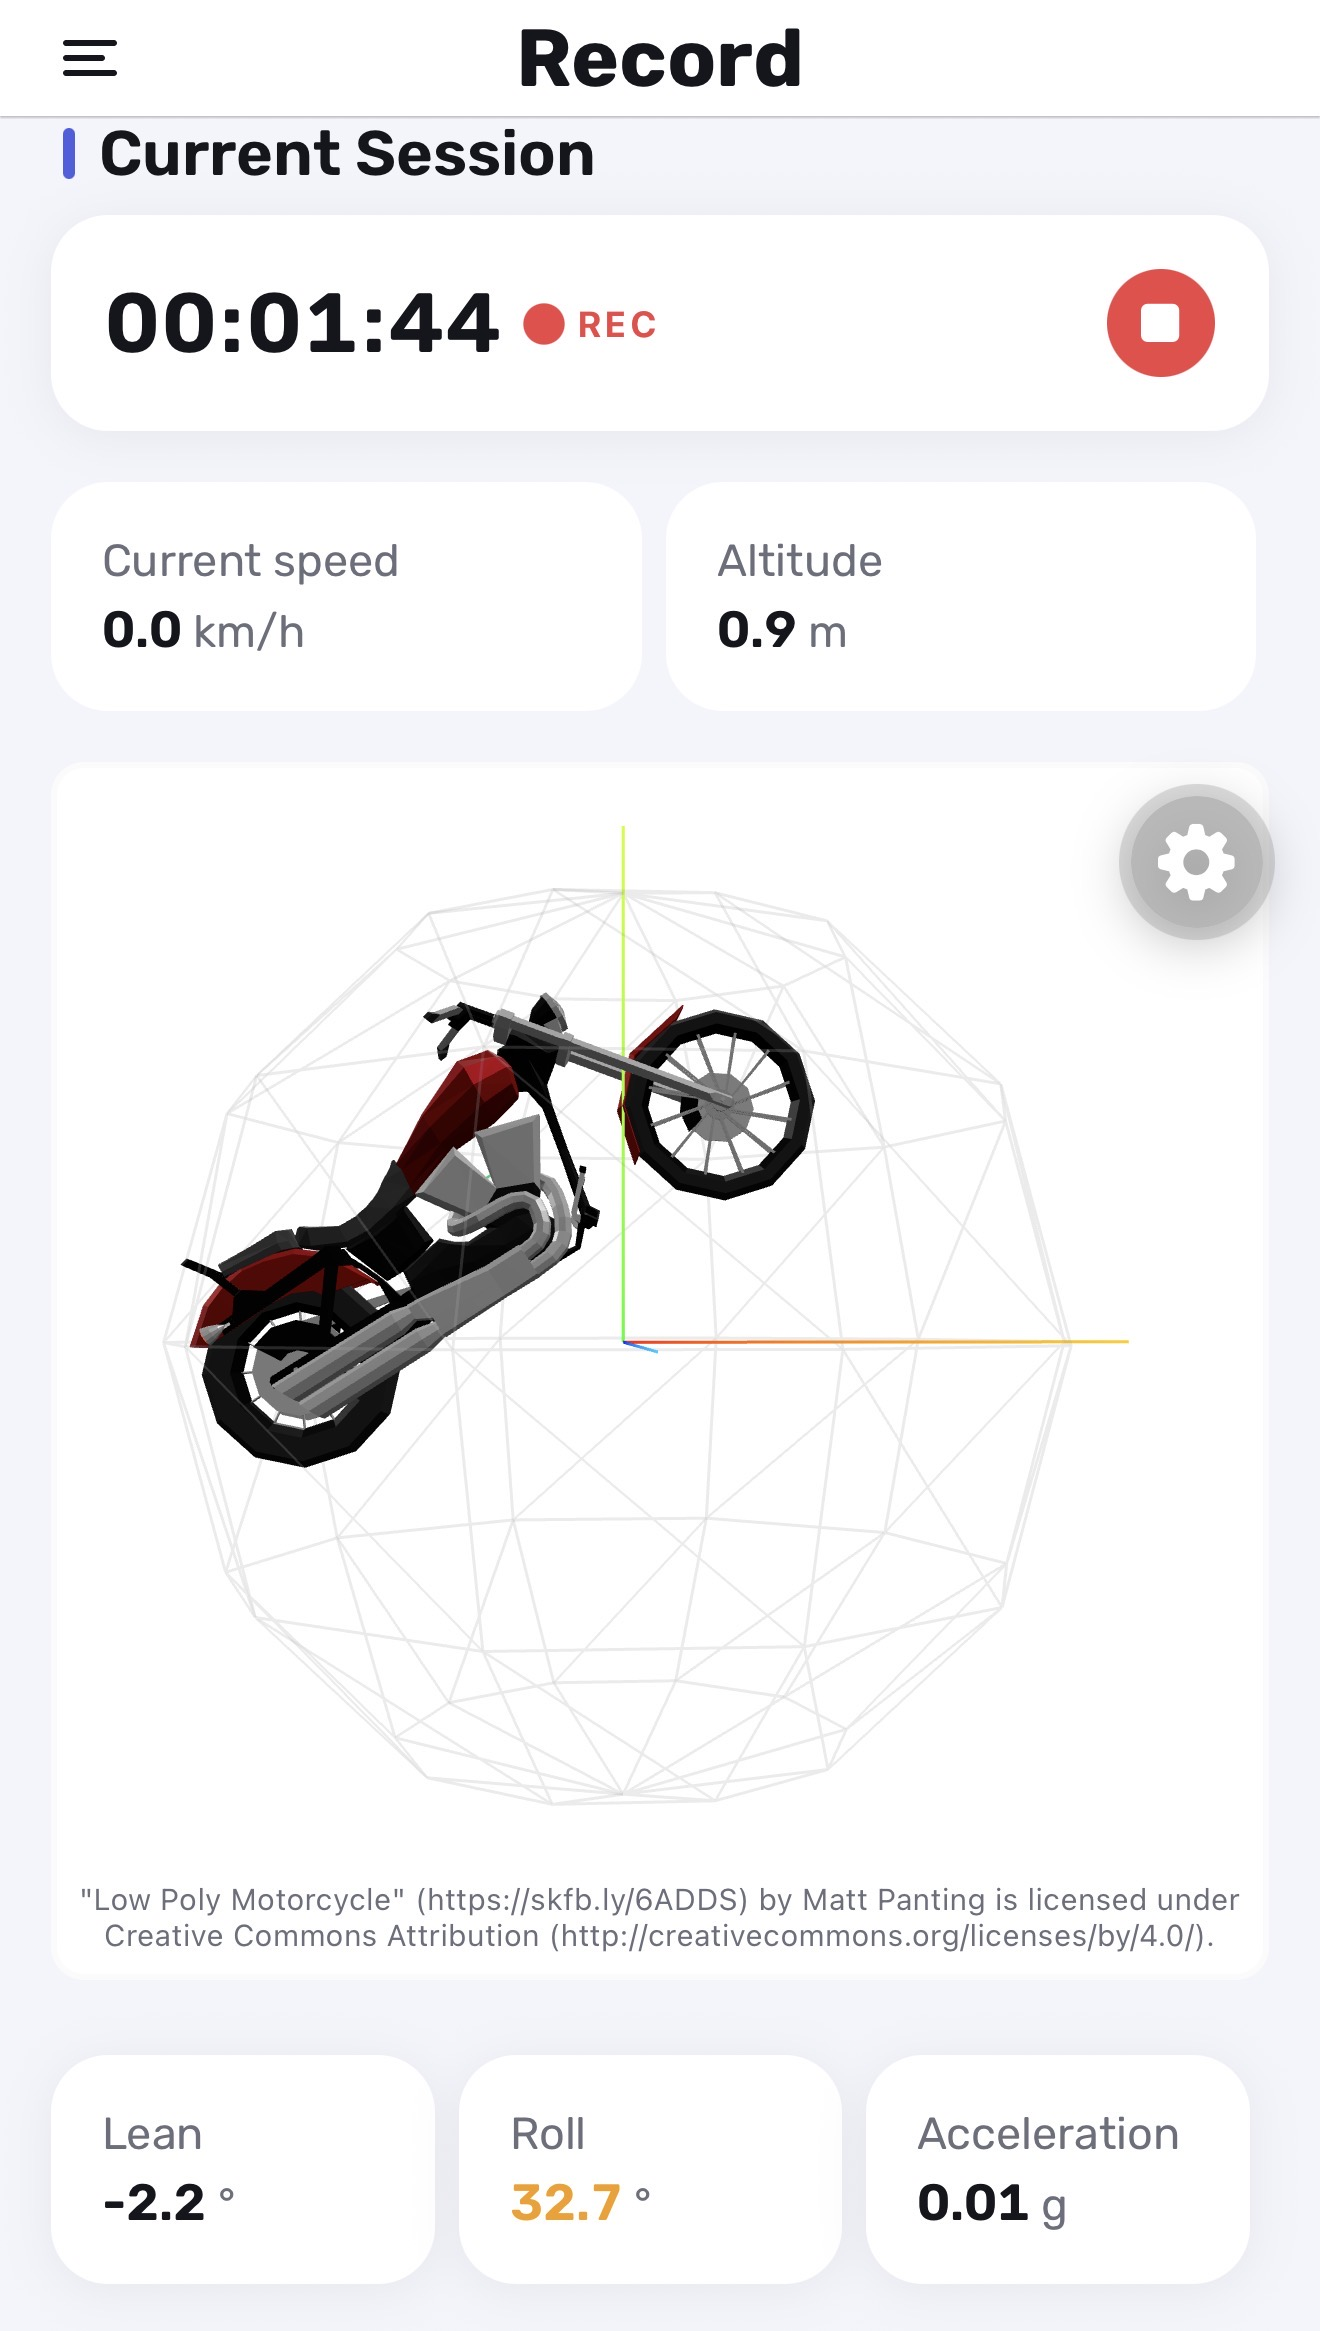
\includegraphics[width=0.62\textwidth]{assets/app_3d_bike.jpeg}
    \end{column}
  \end{columns}
\end{frame}

\section{Verifica e risultati}

\begin{frame}{Verifica e validazione}
  \begin{columns}[T,onlytextwidth]
    \begin{column}{0.5\textwidth}
      \begin{itemize}
        \item \textbf{3 test su campo} su una Yamaha MT-07 reale
        \item Confronto di \textbf{verosimiglianza} con la dinamica di guida
        \item \textbf{2 criticità} individuate e risolte
        \item \textbf{2 test su banco} per inattività e fallback IMU
      \end{itemize}
    \end{column}
    \begin{column}{0.46\textwidth}
      \small
      \begin{tabular}{@{}lc@{}}
        \toprule
        \textbf{Test} & \textbf{Esito} \\
        \midrule
        C-1 Guida su strada & \textcolor{padovapetrol}{\ding{51}} \\
        C-2 Guida su strada & \textcolor{padovapetrol}{\ding{51}} \\
        C-3 Guida su strada & \textcolor{padovared}{\ding{51}*} \\
        B-1 Inattività & \textcolor{padovapetrol}{\ding{51}} \\
        B-2 Fallback IMU & \textcolor{padovapetrol}{\ding{51}} \\
        \bottomrule
      \end{tabular}\\[3pt]
      {\tiny * criticità risolta dopo il test}
    \end{column}
  \end{columns}
\end{frame}

\begin{frame}{Risultati: benchmark prestazionali}
  \begin{columns}[T,onlytextwidth]
    \begin{column}{0.48\textwidth}
      \centering{\scriptsize\bfseries Tempo di scrittura (µs)}\\
      \begin{tikzpicture}
        \begin{axis}[
          ybar,bar width=10pt,width=6.2cm,height=4.1cm,
          symbolic x coords={Media,Massimo},xtick=data,
          ylabel={\tiny µs},ymin=0,
          legend style={font=\tiny,at={(0.5,-0.28)},anchor=north,legend columns=-1},
          tick label style={font=\tiny},
          nodes near coords, every node near coord/.append style={font=\tiny},
          enlarge x limits=0.35]
          \addplot[fill=padovagray] coordinates {(Media,150.045) (Massimo,665.726)};
          \addplot[fill=padovared] coordinates {(Media,83.330) (Massimo,131.747)};
          \legend{Prima,Dopo}
        \end{axis}
      \end{tikzpicture}
    \end{column}
    \begin{column}{0.48\textwidth}
      \centering{\scriptsize\bfseries Occupazione CPU (\%)}\\
      \begin{tikzpicture}
        \begin{axis}[
          ybar,bar width=10pt,width=6.2cm,height=4.1cm,
          symbolic x coords={Prima sess.,Durante sess.},xtick=data,
          ylabel={\tiny \%},ymin=0,ymax=32,
          legend style={font=\tiny,at={(0.5,-0.28)},anchor=north,legend columns=-1},
          tick label style={font=\tiny},
          nodes near coords, every node near coord/.append style={font=\tiny},
          enlarge x limits=0.35]
          \addplot[fill=padovagray] coordinates {(Prima sess.,25) (Durante sess.,25)};
          \addplot[fill=padovared] coordinates {(Prima sess.,3) (Durante sess.,23)};
          \legend{Prima,Dopo}
        \end{axis}
      \end{tikzpicture}
    \end{column}
  \end{columns}
  \vspace{2pt}
  \begin{center}
    \small RAM: \textbf{+6,3\%} \quad$\vert$\quad \textbf{37/38 requisiti} raggiunti complessivamente
  \end{center}
\end{frame}

\section{Conclusioni}

\begin{frame}{Conclusioni}
  \begin{columns}[T,onlytextwidth]
    \begin{column}{0.34\textwidth}
      \centering
      \begin{tikzpicture}
        \draw[line width=6pt,padovagraylight] (0,0) circle (1.35cm);
        \draw[line width=6pt,padovared,line cap=round] (90:1.35cm) arc[start angle=90,end angle=90-360*0.973,radius=1.35cm];
        \node[font=\Large\bfseries,padovared] at (0,0.12) {37/38};
        \node[font=\scriptsize,padovagray] at (0,-0.32) {requisiti};
      \end{tikzpicture}
    \end{column}
    \begin{column}{0.62\textwidth}
      \begin{itemize}
        \item \textbf{37/38 requisiti} raggiunti, tutti gli obiettivi O/D/F
        \item Firmware più \textbf{affidabile, efficiente ed estendibile}
        \item Limiti: \textbf{+6,3\% RAM}, sniffer testato solo su \textbf{Yamaha MT-07}
        \item Crescita personale su \textbf{firmware, FreeRTOS, protocolli CAN/BLE}
      \end{itemize}
    \end{column}
  \end{columns}
\end{frame}

\begin{frame}[plain]
  \begin{tikzpicture}[remember picture, overlay]
    \node[anchor=south east, xshift=-4cm, yshift=0.3cm, opacity=0.3]
      at (current page.south east)
      {
\includegraphics[width=0.53\paperwidth]{assets/logo_unipd_rosso.png}};
  \end{tikzpicture}
  \begin{center}
    \vspace{2.2cm}
    {\usebeamerfont{title}\usebeamercolor[fg]{title}\Huge Grazie per l'attenzione}\\[0.8cm]
    {\color{padovared}\rule{2.6cm}{1.6pt}}\\[0.8cm]
    {\Large\color{padovared}\bfseries Domande?}\\[1.4cm]
  \end{center}
\end{frame}

\end{document}
